\documentclass[a4paper,conference]{IEEEtran}
% This is stripped down to basically the ieee bare_conf.tex header
\usepackage{amssymb,amsmath}
% use upquote if available, for straight quotes in verbatim environments
\IfFileExists{upquote.sty}{\usepackage{upquote}}{}
% use microtype if available
\IfFileExists{microtype.sty}{%
\usepackage{microtype}
\UseMicrotypeSet[protrusion]{basicmath} % disable protrusion for tt fonts
}{}
\usepackage{hyperref}
\PassOptionsToPackage{usenames,dvipsnames}{color} % color is loaded by hyperref
\hypersetup{unicode=true,
            pdftitle={Data Mining- Practice 7 Dimensionality Reduction and PCA},
            pdfborder={0 0 0},
            breaklinks=true}
\urlstyle{same}  % don't use monospace font for urls
% -- biblio. set natbib: true in pandoc for silly hacks around pandoc \cite{} vs \citep{}
\usepackage{cite}
\bibliographystyle{IEEEtran}
\let\citep\cite
% if you want the [2, 3] vs IEEE [2], [3]
\renewcommand{\citepunct}{,\penalty\citepunctpenalty\ }
\usepackage{color}
\usepackage{fancyvrb}
\newcommand{\VerbBar}{|}
\newcommand{\VERB}{\Verb[commandchars=\\\{\}]}
\DefineVerbatimEnvironment{Highlighting}{Verbatim}{commandchars=\\\{\}}
% Add ',fontsize=\small' for more characters per line
\usepackage{framed}
\definecolor{shadecolor}{RGB}{248,248,248}
\newenvironment{Shaded}{\begin{snugshade}}{\end{snugshade}}
\newcommand{\AlertTok}[1]{\textcolor[rgb]{0.94,0.16,0.16}{#1}}
\newcommand{\AnnotationTok}[1]{\textcolor[rgb]{0.56,0.35,0.01}{\textbf{\textit{#1}}}}
\newcommand{\AttributeTok}[1]{\textcolor[rgb]{0.13,0.29,0.53}{#1}}
\newcommand{\BaseNTok}[1]{\textcolor[rgb]{0.00,0.00,0.81}{#1}}
\newcommand{\BuiltInTok}[1]{#1}
\newcommand{\CharTok}[1]{\textcolor[rgb]{0.31,0.60,0.02}{#1}}
\newcommand{\CommentTok}[1]{\textcolor[rgb]{0.56,0.35,0.01}{\textit{#1}}}
\newcommand{\CommentVarTok}[1]{\textcolor[rgb]{0.56,0.35,0.01}{\textbf{\textit{#1}}}}
\newcommand{\ConstantTok}[1]{\textcolor[rgb]{0.56,0.35,0.01}{#1}}
\newcommand{\ControlFlowTok}[1]{\textcolor[rgb]{0.13,0.29,0.53}{\textbf{#1}}}
\newcommand{\DataTypeTok}[1]{\textcolor[rgb]{0.13,0.29,0.53}{#1}}
\newcommand{\DecValTok}[1]{\textcolor[rgb]{0.00,0.00,0.81}{#1}}
\newcommand{\DocumentationTok}[1]{\textcolor[rgb]{0.56,0.35,0.01}{\textbf{\textit{#1}}}}
\newcommand{\ErrorTok}[1]{\textcolor[rgb]{0.64,0.00,0.00}{\textbf{#1}}}
\newcommand{\ExtensionTok}[1]{#1}
\newcommand{\FloatTok}[1]{\textcolor[rgb]{0.00,0.00,0.81}{#1}}
\newcommand{\FunctionTok}[1]{\textcolor[rgb]{0.13,0.29,0.53}{\textbf{#1}}}
\newcommand{\ImportTok}[1]{#1}
\newcommand{\InformationTok}[1]{\textcolor[rgb]{0.56,0.35,0.01}{\textbf{\textit{#1}}}}
\newcommand{\KeywordTok}[1]{\textcolor[rgb]{0.13,0.29,0.53}{\textbf{#1}}}
\newcommand{\NormalTok}[1]{#1}
\newcommand{\OperatorTok}[1]{\textcolor[rgb]{0.81,0.36,0.00}{\textbf{#1}}}
\newcommand{\OtherTok}[1]{\textcolor[rgb]{0.56,0.35,0.01}{#1}}
\newcommand{\PreprocessorTok}[1]{\textcolor[rgb]{0.56,0.35,0.01}{\textit{#1}}}
\newcommand{\RegionMarkerTok}[1]{#1}
\newcommand{\SpecialCharTok}[1]{\textcolor[rgb]{0.81,0.36,0.00}{\textbf{#1}}}
\newcommand{\SpecialStringTok}[1]{\textcolor[rgb]{0.31,0.60,0.02}{#1}}
\newcommand{\StringTok}[1]{\textcolor[rgb]{0.31,0.60,0.02}{#1}}
\newcommand{\VariableTok}[1]{\textcolor[rgb]{0.00,0.00,0.00}{#1}}
\newcommand{\VerbatimStringTok}[1]{\textcolor[rgb]{0.31,0.60,0.02}{#1}}
\newcommand{\WarningTok}[1]{\textcolor[rgb]{0.56,0.35,0.01}{\textbf{\textit{#1}}}}
\usepackage{graphicx,grffile}
\makeatletter
\def\maxwidth{\ifdim\Gin@nat@width>\linewidth\linewidth\else\Gin@nat@width\fi}
\def\maxheight{\ifdim\Gin@nat@height>\textheight\textheight\else\Gin@nat@height\fi}
\makeatother
% Scale images if necessary, so that they will not overflow the page
% margins by default, and it is still possible to overwrite the defaults
% using explicit options in \includegraphics[width, height, ...]{}
\setkeys{Gin}{width=\maxwidth,height=\maxheight,keepaspectratio}

\title{Data Mining- Practice 7 Dimensionality Reduction and PCA}
% for over three affiliations, or if they all won't fit within the width
% of the page, use this alternative format. Cannot use \and or alignment is wrong
\author{\IEEEauthorblockN{%
  Rajesh Kalakoti\IEEEauthorrefmark{4}%
  , Sven Nomm\IEEEauthorrefmark{1}%
}
\IEEEauthorblockA{\IEEEauthorrefmark{1}
      Taltech, Estonia, 12616}
\IEEEauthorblockA{\IEEEauthorrefmark{4}
      Email:
\href{mailto:rajesh.kalakoti@outlook.com}{\nolinkurl{rajesh.kalakoti@outlook.com}}}
}





\date{2023-10-19 14:06:11 +0300}
\setlength{\parindent}{0pt}
\setlength{\parskip}{6pt plus 2pt minus 1pt}
\let\tightlist\relax % silly pandoc thing

% --- user includes
% Put your preamble here. Example.
% subfigures
\usepackage{subfig}
% dots in filenames
\usepackage{graphicx, grffile}
% bold math
\usepackage{bm}
% colours
\usepackage[usenames,dvipsnames]{xcolor}
\usepackage{algpseudocode}
% suppress month in bibliography
%\AtEveryBibitem{\clearfield{month}}
%\AtEveryCitekey{\clearfield{month}}

% texdef -t latex -f {cmdname} to see if cmd is already defined

% Letters in fancy font (expectation, integers, reals, normal dist)
\newcommand{\E}[1]{\operatorname{\mathbb{E}}{\left[#1\right]}}
\newcommand{\Z}{\mathbb{Z}}
\newcommand{\R}{\mathbb{R}}
\newcommand{\N}{\mathcal{N}}

\begin{document}
\maketitle
\begin{abstract}
In today's practical session, we will delve into the core concepts of
data mining. The session is structured to provide a comprehensive
understanding of essential techniques in data preprocessing,
dimensionality reduction, and predictive modeling.
\end{abstract}

\hypertarget{sec:introduction}{%
\section{Introduction}\label{sec:introduction}}

We begin by exploring the significance of data normalization, a crucial
preprocessing step in data mining. Normalization ensures that features
are on a consistent scale, facilitating accurate comparisons and
analyses. Through hands-on exercises, attendees will learn various
normalization techniques in R, enabling them to prepare diverse datasets
for effective mining.

\hypertarget{sec:missing-entries}{%
\subsection{Missing Entries}\label{sec:missing-entries}}

Handling missing entries in a dataset is also called Data imputation.
Data imputation is a statistical technique used to fill in missing or
incomplete data points within a dataset.

\hypertarget{sec:mean-median-or-mode-imputation}{%
\subsubsection{Mean, Median, or Mode
Imputation}\label{sec:mean-median-or-mode-imputation}}

Missing values are replaced by the mean (average), median, or mode (most
frequently occurring value) of the observed data for the respective
variable.

\hypertarget{sec:regression-imputation}{%
\subsubsection{Regression Imputation}\label{sec:regression-imputation}}

Missing values are predicted using regression models based on other
variables in the dataset. A regression equation is created using
variables without missing data, and this equation is used to estimate
the missing values.

\hypertarget{sec:k-nearest-neighbors-knn-imputation}{%
\subsubsection{K-Nearest Neighbors (KNN)
Imputation}\label{sec:k-nearest-neighbors-knn-imputation}}

Missing values are imputed based on values from similar cases
(neighbors) in the dataset. The KNN algorithm identifies the nearest
neighbors for each missing value and imputes the missing value based on
their values.

\hypertarget{sec:multiple-imputation}{%
\subsubsection{Multiple Imputation}\label{sec:multiple-imputation}}

Multiple imputation involves creating multiple complete versions of the
dataset, each with different imputed values. Statistical analyses are
then performed on each dataset, and the results are combined to account
for the uncertainty introduced by imputation.

\hypertarget{sec:data-normalization}{%
\section{Data Normalization}\label{sec:data-normalization}}

Data normalization is a type of data preprocessing technique that
focuses on transforming features to a similar scale.

\hypertarget{sec:z-score-normalization-standardization}{%
\subsection{z-Score Normalization
(Standardization):}\label{sec:z-score-normalization-standardization}}

Z-score normalization standardizes the data by transforming it to have
zero mean and unit variance.

\[
z^j_{i} = \frac{(x^j_{i}  - \mu_j)}{\sigma_j} 
\] - \(x\) is the original value, - \(\mu\) is the mean of the variable,
- \(\sigma\) is the standard deviation of the variable.

\hypertarget{sec:min-max-normalization}{%
\subsection{min-max normalization}\label{sec:min-max-normalization}}

Min-max scaling transforms the data within range {[}0, 1{]}.

\[
y^j_{i} = \frac{x^j_{i} - \min(x^j)}{\max(x^j) - \min(x^j)}
\]

\hypertarget{sec:code-for-data-data-normalization}{%
\subsubsection{Code for data Data
normalization}\label{sec:code-for-data-data-normalization}}

Here is the below function are written for two normalization techniques.
Min-max normalization is useful when the data has a fixed range. Deep
learning based models mostly recommended data normalization because of
gradient descent.

\begin{Shaded}
\begin{Highlighting}[]
\NormalTok{z\_score }\OtherTok{\textless{}{-}} \ControlFlowTok{function}\NormalTok{(x) \{}
  \ControlFlowTok{if}\NormalTok{ (}\FunctionTok{is.numeric}\NormalTok{(x)) \{}
\NormalTok{    mean\_x }\OtherTok{\textless{}{-}} \FunctionTok{mean}\NormalTok{(x)}
\NormalTok{    sd\_x }\OtherTok{\textless{}{-}} \FunctionTok{sd}\NormalTok{(x)}
\NormalTok{    std\_values }\OtherTok{\textless{}{-}}\NormalTok{ (x }\SpecialCharTok{{-}}\NormalTok{ mean\_x) }\SpecialCharTok{/}\NormalTok{ sd\_x}
    \FunctionTok{return}\NormalTok{(std\_values)}
\NormalTok{  \} }\ControlFlowTok{else} \ControlFlowTok{if}\NormalTok{ (}\FunctionTok{is.matrix}\NormalTok{(x) }\SpecialCharTok{||} \FunctionTok{is.data.frame}\NormalTok{(x)) \{}
\NormalTok{    std\_matrix }\OtherTok{\textless{}{-}} \FunctionTok{scale}\NormalTok{(x)}
    \FunctionTok{return}\NormalTok{(std\_matrix)}
\NormalTok{  \} }\ControlFlowTok{else}\NormalTok{ \{}
    \FunctionTok{stop}\NormalTok{(}\StringTok{"Unsupported input type"}\NormalTok{)}
\NormalTok{  \}}
\NormalTok{\}}

\CommentTok{\# Load the iris dataset}
\FunctionTok{data}\NormalTok{(iris)}
\NormalTok{z\_score\_iris }\OtherTok{\textless{}{-}} \FunctionTok{z\_score}\NormalTok{(iris[, }\DecValTok{1}\SpecialCharTok{:}\DecValTok{4}\NormalTok{])}
\end{Highlighting}
\end{Shaded}

\begin{Shaded}
\begin{Highlighting}[]
\FunctionTok{print}\NormalTok{(}\FunctionTok{xtable}\NormalTok{(}
    \FunctionTok{head}\NormalTok{(z\_score\_iris),}
    \AttributeTok{caption=}\StringTok{\textquotesingle{}Table showing z{-}score normalization top 5 rows.\textquotesingle{}}\NormalTok{,}
    \AttributeTok{label=}\StringTok{\textquotesingle{}tbl:xtable.floating\textquotesingle{}}\NormalTok{),}
    \AttributeTok{align=}\FunctionTok{c}\NormalTok{(}\FunctionTok{rep}\NormalTok{(}\StringTok{\textquotesingle{}r\textquotesingle{}}\NormalTok{, }\DecValTok{6}\NormalTok{), }\StringTok{\textquotesingle{}l\textquotesingle{}}\NormalTok{))}
\end{Highlighting}
\end{Shaded}

\begin{table}[!t]
\centering
\caption{Table showing z-score normalization top 5 rows.} 
\label{tbl:xtable.floating}
\begin{tabular}{rrrr}
  \hline
Sepal.Length & Sepal.Width & Petal.Length & Petal.Width \\ 
  \hline
-0.90 & 1.02 & -1.34 & -1.31 \\ 
  -1.14 & -0.13 & -1.34 & -1.31 \\ 
  -1.38 & 0.33 & -1.39 & -1.31 \\ 
  -1.50 & 0.10 & -1.28 & -1.31 \\ 
  -1.02 & 1.25 & -1.34 & -1.31 \\ 
  -0.54 & 1.93 & -1.17 & -1.05 \\ 
   \hline
\end{tabular}
\end{table}

\begin{Shaded}
\begin{Highlighting}[]
\NormalTok{min\_max }\OtherTok{\textless{}{-}} \ControlFlowTok{function}\NormalTok{(x) \{}
  \ControlFlowTok{if}\NormalTok{ (}\FunctionTok{is.numeric}\NormalTok{(x)) \{}
\NormalTok{    min\_x }\OtherTok{\textless{}{-}} \FunctionTok{min}\NormalTok{(x)}
\NormalTok{    max\_x }\OtherTok{\textless{}{-}} \FunctionTok{max}\NormalTok{(x)}
\NormalTok{    min\_max }\OtherTok{\textless{}{-}}\NormalTok{ (x }\SpecialCharTok{{-}}\NormalTok{ min\_x)}\SpecialCharTok{/}\NormalTok{(max\_x }\SpecialCharTok{{-}}\NormalTok{ min\_x)}
    \FunctionTok{return}\NormalTok{(min\_max)}
\NormalTok{  \} }\ControlFlowTok{else} \ControlFlowTok{if}\NormalTok{(}\FunctionTok{is.matrix}\NormalTok{(x) }\SpecialCharTok{||} \FunctionTok{is.data.frame}\NormalTok{(x))}
\NormalTok{    \{}
\NormalTok{    normalized\_matrix }\OtherTok{\textless{}{-}} \FunctionTok{as.data.frame}\NormalTok{(}
      \FunctionTok{lapply}\NormalTok{(x, min\_max\_normalize))}
    \FunctionTok{return}\NormalTok{(normalized\_matrix)}
\NormalTok{  \} }\ControlFlowTok{else}\NormalTok{ \{}
    \FunctionTok{stop}\NormalTok{(}\StringTok{"Unsupported input type"}\NormalTok{)}
\NormalTok{  \}}
\NormalTok{\}}
\NormalTok{x }\OtherTok{\textless{}{-}} \FunctionTok{c}\NormalTok{(}\DecValTok{2}\NormalTok{, }\DecValTok{5}\NormalTok{, }\DecValTok{8}\NormalTok{, }\DecValTok{3}\NormalTok{, }\DecValTok{10}\NormalTok{)}
\NormalTok{normalized\_x }\OtherTok{\textless{}{-}} \FunctionTok{min\_max}\NormalTok{(x)}
\FunctionTok{print}\NormalTok{(normalized\_x)}
\end{Highlighting}
\end{Shaded}

\begin{verbatim}
## [1] 0.000 0.375 0.750 0.125 1.000
\end{verbatim}

\hypertarget{sec:dimensionality-reduction}{%
\section{Dimensionality Reduction}\label{sec:dimensionality-reduction}}

Let the data \textbf{D} consist of \emph{n} points over \emph{d}
attributes, that is, it is an \emph{n × d} matrix.

Principal Component Analysis (PCA) is a technique that seeks a \(r\)
-dimensional basis that best captures the variance in the data. The
direction with the largest projected variance is called the first
principal component. The orthogonal direction that captures the second
largest projected variance is called the second principal component, and
so on.

\[PCA(D, \alpha)\]

\begin{enumerate}
\def\labelenumi{\arabic{enumi}.}
\item
  \textbf{Compute the Mean:} \[
  \mu = \frac{1}{n} \sum_{i=1}^{n} x_i
  \] Compute the mean of the dataset.
\item
  \textbf{Center the Data:} \[
  \overline{D} = D - 1 \cdot \mu^T
  \] Center the data by subtracting the mean from each data point.
\item
  \textbf{Compute the Covariance Matrix:} \[
  \sum = \frac{1}{n} (\overline{D}^T \overline{D})
  \] Compute the covariance matrix.
\item
  \textbf{Compute Eigenvalues (\(\sum\)):}
\end{enumerate}

\[
(\lambda_1, \lambda_2, \ldots, \lambda_d)
\]

compute eigen values of co-variance matrix

\begin{enumerate}
\def\labelenumi{\arabic{enumi}.}
\setcounter{enumi}{4}
\item
  \textbf{Compute Eigen vectors (\(\sum\)):}. \[
  U = (u_1, u_2,... u_d)
  \] compute eigen vectors of co-variance matrix.
\item
  \textbf{Compute Fraction of Total Variance (\(f(r)\)):} \[
  f(r) = \frac{\sum_{i=1}^{r} \lambda_i}{\sum_{i=1}^{d} \lambda_i}, \quad \text{for all } r = 1, 2, \ldots, d
  \] Compute the fraction of total variance for each dimension.
\item
  \textbf{Choose Smallest \(r\) such that \(f(r) \geq \alpha\):} Choose
  the dimensionality \(r\) such that the fraction of total variance is
  greater than or equal to the specified threshold (\(\alpha\)).
\item
  \textbf{Reduce Eigenvectors (\(U_r\)):} \[
  U_r = \begin{pmatrix} u_1 & u_2 & \ldots & u_r \end{pmatrix}
  \] Select the first \(r\) eigenvectors to form the reduced basis.
\item
  \textbf{Transform Data (\(A\)):} \[
  A = \left\{ a_i \, \middle| \, a_i = U_r^T \overline{x}_i, \text{ for } i = 1, \ldots, n \right\}
  \]
\end{enumerate}

Obtain the reduced dimensionality data by multiplying the reduced basis
(\(U_r^T\)) with the original data (\(x_i\)) for \(i = 1, \ldots, n\).

\begin{Shaded}
\begin{Highlighting}[]
\NormalTok{pca }\OtherTok{\textless{}{-}} \ControlFlowTok{function}\NormalTok{(}
\NormalTok{    D, alpha, num\_components) \{}
  \CommentTok{\# Step 1: Compute the mean}
\NormalTok{  mu }\OtherTok{\textless{}{-}} \FunctionTok{colMeans}\NormalTok{(D)}
  
  \CommentTok{\# Step 2: Center the data}
\NormalTok{  D\_centered }\OtherTok{\textless{}{-}}\NormalTok{ D }\SpecialCharTok{{-}} \FunctionTok{matrix}\NormalTok{(mu, }\FunctionTok{nrow}\NormalTok{(D), }
                           \FunctionTok{ncol}\NormalTok{(D),}
                           \AttributeTok{byrow =} \ConstantTok{TRUE}\NormalTok{)}
  
  \CommentTok{\# Step 3: Computethe covariance matrix}
\NormalTok{  cov\_matrix }\OtherTok{\textless{}{-}} \FunctionTok{cov}\NormalTok{(D\_centered)}
  
  \CommentTok{\# Step 4: Compute eigenvalues}
  \CommentTok{\# and eigenvectors}
\NormalTok{  eig\_result }\OtherTok{\textless{}{-}} \FunctionTok{eigen}\NormalTok{(cov\_matrix)}
\NormalTok{  eig\_val }\OtherTok{\textless{}{-}}\NormalTok{ eig\_result}\SpecialCharTok{$}\NormalTok{values}
\NormalTok{  eig\_vect }\OtherTok{\textless{}{-}}\NormalTok{ eig\_result}\SpecialCharTok{$}\NormalTok{vectors}
  
  \CommentTok{\# Step 5: Compute fraction of total variance}
\NormalTok{  tot\_var }\OtherTok{\textless{}{-}} \FunctionTok{sum}\NormalTok{(eig\_val)}
\NormalTok{  var\_frac }\OtherTok{\textless{}{-}} \FunctionTok{cumsum}\NormalTok{(eig\_val)}\SpecialCharTok{/}\NormalTok{tot\_var}

  \CommentTok{\# Step 6: Choose components }
  \CommentTok{\# based on alpha}
\NormalTok{  num\_components }\OtherTok{\textless{}{-}} \FunctionTok{min}\NormalTok{(}\FunctionTok{which}\NormalTok{(var\_frac}
                              \SpecialCharTok{\textgreater{}=}\NormalTok{ alpha))}
  
  \CommentTok{\# Step 7: Reduce eigenvectors}
\NormalTok{  red\_basis }\OtherTok{\textless{}{-}}\NormalTok{ eig\_vect[, }\DecValTok{1}\SpecialCharTok{:}\NormalTok{num\_components]}
  
  \CommentTok{\# Step 8: Transform data}
\NormalTok{  red\_data }\OtherTok{\textless{}{-}} \FunctionTok{as.matrix}\NormalTok{(D\_centered) }\SpecialCharTok{\%*\%}\NormalTok{ red\_basis}
  
  \FunctionTok{return}\NormalTok{(red\_data)}
\NormalTok{\}}



\CommentTok{\# Test PCA on iris dataset, }
\CommentTok{\#reducing from 4 features to 2 }
\CommentTok{\#features with alpha=0.95}
\FunctionTok{library}\NormalTok{(datasets)}

\CommentTok{\# Load iris dataset}
\FunctionTok{data}\NormalTok{(iris)}

\CommentTok{\# Extract features from iris dataset}
\NormalTok{features }\OtherTok{\textless{}{-}}\NormalTok{ iris[, }\DecValTok{1}\SpecialCharTok{:}\DecValTok{4}\NormalTok{]}

\CommentTok{\# Perform PCA with alpha=0.95 }
\CommentTok{\#and 2 components}
\NormalTok{reduced\_data }\OtherTok{\textless{}{-}} \FunctionTok{pca}\NormalTok{(}
\NormalTok{  features, }\AttributeTok{alpha =} \FloatTok{0.95}\NormalTok{, }
  \AttributeTok{num\_components =} \DecValTok{2}\NormalTok{)}

\CommentTok{\# Plot PCA results with }
\CommentTok{\# customized axis labels}
\FunctionTok{plot}\NormalTok{(reduced\_data, }\AttributeTok{col =}\NormalTok{ iris}\SpecialCharTok{$}\NormalTok{Species, }
     \AttributeTok{pch =} \DecValTok{16}\NormalTok{, }
     \AttributeTok{main =} \StringTok{"PCA of Iris Dataset"}\NormalTok{,}
     \AttributeTok{xlab =} \StringTok{"Dim 1"}\NormalTok{, }\AttributeTok{ylab =} \StringTok{"Dim 2"}\NormalTok{)}
\FunctionTok{legend}\NormalTok{(}\StringTok{"topright"}\NormalTok{,}
       \AttributeTok{legend =} \FunctionTok{levels}\NormalTok{(iris}\SpecialCharTok{$}\NormalTok{Species),}
       \AttributeTok{col =} \DecValTok{1}\SpecialCharTok{:}\DecValTok{3}\NormalTok{,}
       \AttributeTok{pch =} \DecValTok{16}\NormalTok{)}
\end{Highlighting}
\end{Shaded}

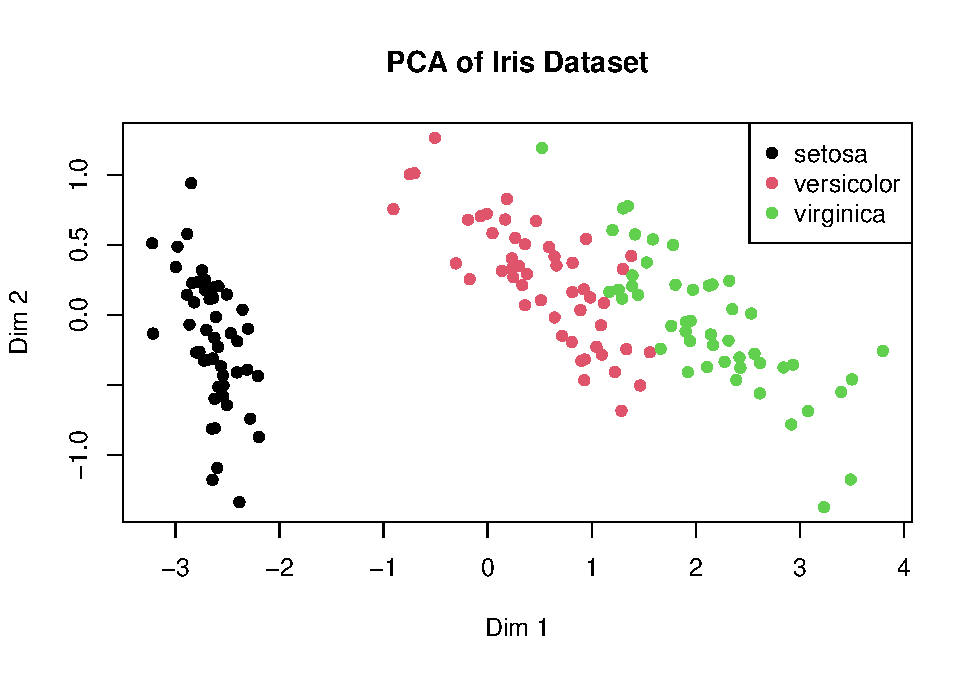
\includegraphics{figure/unnamed-chunk-3-1.pdf}

\hypertarget{sec:linear-regression}{%
\section{Linear Regression}\label{sec:linear-regression}}

Given a set of attributes or variables \(X_1\), \(X_2\), \ldots,
\(X_d\), called the predictor, explanatory, or independent variables,
and given a real-valued attribute of interest \(Y\), called the response
or dependent variable, the aim of regression is to predict the response
variable based on the independent variables. That is, the goal is to
learn a regression function \(f\), such that

\[ Y = f(X_1, X_2, ..., X_d) + \epsilon = f(X) + \epsilon \]

where \(X = (X_1, X_2, ..., X_d)^T\) is the multivariate random variable
comprising the predictor attributes, and \(\epsilon\) is a random error
term that is assumed to be independent of \(X\). In other words, \(Y\)
is comprised of two components, one dependent on the observed predictor
attributes, and the other, coming from the error term, independent of
the predictor attributes. The error term encapsulates inherent
uncertainty in \(Y\), as well as, possibly the effect of unobserved,
hidden or latent variables.

\hypertarget{sec:linear-regression-model}{%
\subsection{LINEAR REGRESSION MODEL}\label{sec:linear-regression-model}}

In linear regression, the function \(f\) is assumed to be linear in its
parameters. It can be represented as:

\[ 
f(X) = \beta + \omega_1 X_1 + \omega_2 X_2 + \ldots + \omega_d X_d = \beta + \sum_{i=1}^{d} \omega_i X_i = \beta + \omega^T X 
\] Here, the parameter \(\beta\) is the true (unknown) bias term, the
parameter \(\omega_i\) is the true (unknown) regression coefficient or
weight for attribute \(X_i\), and
\(\omega = (\omega_1, \omega_2, \ldots, \omega_d)^T\) is the true
d-dimensional weight vector.

\hypertarget{sec:bivariate-regression}{%
\subsubsection{BIVARIATE REGRESSION}\label{sec:bivariate-regression}}

Let us first consider the case where the input data \(D\) comprises a
single predictor attribute, \(X = (x_1, x_2, \ldots, x_n)^T\), along
with the response variable, \(Y = (y_1, y_2, \ldots, y_n)^T\). Since
\(f\) is linear, we have:

\[
\hat{y}_i = f(x_i) = b + w \cdot x_i
\]

Thus, we seek the straight line \(f(x)\) with slope \(w\) and intercept
\(b\) that best fits the data. The residual error, which is the
difference between the predicted value (also called the fitted value)
and the observed value of the response variable, is given as:

\[ 
\epsilon_i = y_i - \hat{y}_i 
\]

Note that \(|\epsilon|\) denotes the vertical distance between the
fitted and observed response. The best-fitting line minimizes the sum of
squared errors.

\[ 
\text{min}_{b, w} \text{SSE} = \sum_{i=1}^{n} \epsilon_i^2 = \sum_{i=1}^{n} (y_i - \hat{y}_i)^2 = \sum_{i=1}^{n} (y_i - b - w \cdot x_i)^2 
\]

To solve this objective, we differentiate it with respect to \(b\) and
set the result to 0 to obtain:

\[ 
\frac{\partial \text{SSE}}{\partial b} = -2 \sum_{i=1}^{n} (y_i - b - w \cdot x_i) = 0 \quad  
\]

\[ 
w = \frac{(\sum_{i=1}^{n} x_i \cdot y_i) - n \cdot \mu_X \cdot \mu_Y}{\sum_{i=1}^{n} x_i^2 - n \cdot \mu^2_X} 
\]

The regression coefficient \(w\) can also be written as

\[ w = \frac{\sum_{i=1}^{n} (x_i - \mu_X)(y_i - \mu_Y)}{\sum_{i=1}^{n} (x_i - \mu_X)^2} = \frac{\sigma_{XY}}{\sigma_X^2} = \frac{\text{cov}(X, Y)}{\text{var}(X)} 
\]

where \(\sigma_X^2\) is the variance of \(X\), and \(\sigma_{XY}\) is
the covariance between \(X\) and \(Y\). Noting that the correlation
between \(X\) and \(Y\) is given as
\(\rho_{XY} = \frac{\sigma_{XY}}{\sigma_X \cdot \sigma_Y}\), we can also
express \(w\) as:

\[
w = \rho_{XY} \cdot \frac{\sigma_Y}{\sigma_X} 
\]

\hypertarget{sec:code-for-linear-regression}{%
\subsubsection{Code For LInear
regression}\label{sec:code-for-linear-regression}}

Here I have created sample for regression exmaple, you can check the
sample dataset csv file with regression\_data in data folder.

\begin{Shaded}
\begin{Highlighting}[]
\FunctionTok{library}\NormalTok{(here)}
\end{Highlighting}
\end{Shaded}

\begin{verbatim}
## here() starts at /home/rajeshkalakoti/Documents/data_mining_with_R
\end{verbatim}

\begin{Shaded}
\begin{Highlighting}[]
\NormalTok{data\_file }\OtherTok{=} \FunctionTok{here}\NormalTok{(}\StringTok{"data"}\NormalTok{, }
                 \StringTok{"regression\_data.csv"}\NormalTok{);}
\NormalTok{data }\OtherTok{=} \FunctionTok{read.csv}\NormalTok{(data\_file,}\AttributeTok{header=}\ConstantTok{TRUE}\NormalTok{)}
\FunctionTok{dim}\NormalTok{(data)}
\end{Highlighting}
\end{Shaded}

\begin{verbatim}
## [1] 1000    6
\end{verbatim}

\begin{Shaded}
\begin{Highlighting}[]
\CommentTok{\# random simple using sample()}
\NormalTok{row.number }\OtherTok{\textless{}{-}} \FunctionTok{sample}\NormalTok{(}\DecValTok{1}\SpecialCharTok{:}\FunctionTok{nrow}\NormalTok{(data),}
                     \FloatTok{0.8}\SpecialCharTok{*}\FunctionTok{nrow}\NormalTok{(data)) }
\CommentTok{\# 800 observation to train the data}
\NormalTok{training }\OtherTok{=}\NormalTok{ data[row.number,]}
 \CommentTok{\# 200 observation to test the data}
\NormalTok{testing }\OtherTok{=}\NormalTok{ data[}\SpecialCharTok{{-}}\NormalTok{row.number,]}
\CommentTok{\# dimension of training data,}
\CommentTok{\#800 rows with 6 variables}
\FunctionTok{dim}\NormalTok{(training)    }
\end{Highlighting}
\end{Shaded}

\begin{verbatim}
## [1] 800   6
\end{verbatim}

\begin{Shaded}
\begin{Highlighting}[]
\FunctionTok{dim}\NormalTok{(testing)  }
\end{Highlighting}
\end{Shaded}

\begin{verbatim}
## [1] 200   6
\end{verbatim}

\begin{Shaded}
\begin{Highlighting}[]
\CommentTok{\# select all X\textquotesingle{}s column for training }
\NormalTok{trainingX }\OtherTok{\textless{}{-}} \FunctionTok{subset}\NormalTok{(training, }
                    \AttributeTok{select =} \SpecialCharTok{{-}}\FunctionTok{c}\NormalTok{(Y)) }
\CommentTok{\# select only Y column for training}
\NormalTok{trainingY }\OtherTok{\textless{}{-}} \FunctionTok{subset}\NormalTok{(training,}
                    \AttributeTok{select =} \FunctionTok{c}\NormalTok{(Y)) }
 \CommentTok{\# select all X\textquotesingle{}s column for testing}
\NormalTok{testingX }\OtherTok{\textless{}{-}} \FunctionTok{subset}\NormalTok{(testing,}
                   \AttributeTok{select =} \SpecialCharTok{{-}}\FunctionTok{c}\NormalTok{(Y))}
\CommentTok{\# select only Y column for testing}
\NormalTok{testingY }\OtherTok{\textless{}{-}} \FunctionTok{subset}\NormalTok{(testing, }
                   \AttributeTok{select =} \FunctionTok{c}\NormalTok{(Y)) }
\end{Highlighting}
\end{Shaded}

\begin{Shaded}
\begin{Highlighting}[]
\NormalTok{linearRegression }\OtherTok{\textless{}{-}} \ControlFlowTok{function}\NormalTok{(x,y) }
\NormalTok{  \{ }\CommentTok{\# create a function of x and y data}
  \CommentTok{\# vector of 1\textquotesingle{}s with the }
  \CommentTok{\#same amount af rows.}
\NormalTok{  intercept }\OtherTok{\textless{}{-}} \FunctionTok{rep}\NormalTok{(}\DecValTok{1}\NormalTok{, }\FunctionTok{nrow}\NormalTok{(x))}
  \CommentTok{\# Add intercept column to x}
\NormalTok{  x }\OtherTok{\textless{}{-}} \FunctionTok{cbind}\NormalTok{(intercept, x)}
  \CommentTok{\# create x matrix of feature variables}
\NormalTok{  matrix\_X }\OtherTok{\textless{}{-}} \FunctionTok{as.matrix}\NormalTok{(x) }
  \CommentTok{\# create y vector of }
  \CommentTok{\#  the response variable}
\NormalTok{  vector\_Y }\OtherTok{\textless{}{-}} \FunctionTok{as.matrix}\NormalTok{(y) }
\NormalTok{  betas  }\OtherTok{\textless{}{-}} \FunctionTok{solve}\NormalTok{(}
    \FunctionTok{t}\NormalTok{(matrix\_X) }\SpecialCharTok{\%*\%}\NormalTok{ matrix\_X) }\SpecialCharTok{\%*\%} \FunctionTok{t}\NormalTok{(}
\NormalTok{      matrix\_X) }\SpecialCharTok{\%*\%}\NormalTok{ vector\_Y}
\NormalTok{  betas }\OtherTok{\textless{}{-}} \FunctionTok{round}\NormalTok{(betas, }\DecValTok{2}\NormalTok{)}
  \FunctionTok{return}\NormalTok{(betas) }
\NormalTok{\}}

\NormalTok{PredictY }\OtherTok{\textless{}{-}} \ControlFlowTok{function}\NormalTok{(x, betas) \{}
\NormalTok{  betas\_matrix }\OtherTok{\textless{}{-}} \FunctionTok{t}\NormalTok{(}\FunctionTok{as.matrix}\NormalTok{(betas)) }
\NormalTok{  intercept }\OtherTok{\textless{}{-}} \FunctionTok{rep}\NormalTok{(}\DecValTok{1}\NormalTok{, }\FunctionTok{nrow}\NormalTok{(x))   }
\NormalTok{  x }\OtherTok{\textless{}{-}} \FunctionTok{cbind}\NormalTok{(intercept, x)   }
\NormalTok{  matrix\_X }\OtherTok{\textless{}{-}} \FunctionTok{t}\NormalTok{(}\FunctionTok{as.matrix}\NormalTok{(x))}
\NormalTok{  Ŷ }\OtherTok{\textless{}{-}}\NormalTok{ betas\_matrix }\SpecialCharTok{\%*\%}\NormalTok{ matrix\_X}
  \FunctionTok{return}\NormalTok{(Ŷ)}
\NormalTok{\} }
\end{Highlighting}
\end{Shaded}

Error function

\begin{Shaded}
\begin{Highlighting}[]
\NormalTok{errors }\OtherTok{\textless{}{-}} \ControlFlowTok{function}\NormalTok{(Y, Ŷ)\{}
\NormalTok{  Y }\OtherTok{\textless{}{-}} \FunctionTok{as.matrix}\NormalTok{(Y)}
\NormalTok{  Ŷ }\OtherTok{\textless{}{-}} \FunctionTok{t}\NormalTok{(}\FunctionTok{as.matrix}\NormalTok{(Ŷ))}
  \CommentTok{\# compute the sum squared errors}
\NormalTok{  RSS }\OtherTok{=} \FunctionTok{sum}\NormalTok{((Y}\SpecialCharTok{{-}}\NormalTok{ Ŷ)}\SpecialCharTok{\^{}}\DecValTok{2}\NormalTok{)  }
  \CommentTok{\# RSS gives a measure of }
  \CommentTok{\# error of prediction, }
  \CommentTok{\#the lower it is the more our model }
  \CommentTok{\#is accurate }
  \CommentTok{\# compute the }
  \CommentTok{\#total sum of squares}
\NormalTok{  TSS }\OtherTok{=} \FunctionTok{sum}\NormalTok{((Y }\SpecialCharTok{{-}} \FunctionTok{mean}\NormalTok{(Ŷ))}\SpecialCharTok{\^{}}\DecValTok{2}\NormalTok{)}
  \CommentTok{\# R2 represents }
  \CommentTok{\#the proportion of variance}
\NormalTok{  R2 }\OtherTok{\textless{}{-}} \DecValTok{1} \SpecialCharTok{{-}}\NormalTok{ (RSS}\SpecialCharTok{/}\NormalTok{TSS) }
  \CommentTok{\# Root mean square error }
  \CommentTok{\# we will use it to evaluate our model}
\NormalTok{  RMSE }\OtherTok{\textless{}{-}} \FunctionTok{sqrt}\NormalTok{(}\FunctionTok{mean}\NormalTok{((Ŷ }\SpecialCharTok{{-}}\NormalTok{ Y)}\SpecialCharTok{\^{}}\DecValTok{2}\NormalTok{)) }
  \CommentTok{\# return list of R2 and RMSE}
  \FunctionTok{return}\NormalTok{(}\FunctionTok{list}\NormalTok{(}\AttributeTok{R2 =}\NormalTok{ R2, }
              \AttributeTok{RMSE =}\NormalTok{ RMSE,}
              \AttributeTok{RSS =}\NormalTok{ RSS, }\AttributeTok{TSS =}\NormalTok{ TSS)) }
\NormalTok{\}}
\end{Highlighting}
\end{Shaded}

\begin{Shaded}
\begin{Highlighting}[]
\NormalTok{betas }\OtherTok{\textless{}{-}} \FunctionTok{linearRegression}\NormalTok{(}
\NormalTok{  trainingX,trainingY)}
\CommentTok{\# dimension of betas}
\CommentTok{\#is 6 values of Y intercept}
\FunctionTok{dim}\NormalTok{(betas) }
\end{Highlighting}
\end{Shaded}

\begin{verbatim}
## [1] 6 1
\end{verbatim}

\begin{Shaded}
\begin{Highlighting}[]
\FunctionTok{print}\NormalTok{(betas)}
\end{Highlighting}
\end{Shaded}

\begin{verbatim}
##               Y
## intercept  2.12
## X1         0.01
## X2         0.00
## X3        -1.30
## X4         0.39
## X5         2.09
\end{verbatim}

\begin{Shaded}
\begin{Highlighting}[]
\CommentTok{\# compute Ŷ with PredictY function using }
\NormalTok{Ŷ }\OtherTok{\textless{}{-}} \FunctionTok{PredictY}\NormalTok{(testingX,}
\NormalTok{              betas)}
\FunctionTok{dim}\NormalTok{(Ŷ) }
\end{Highlighting}
\end{Shaded}

\begin{verbatim}
## [1]   1 200
\end{verbatim}

\begin{Shaded}
\begin{Highlighting}[]
\NormalTok{error }\OtherTok{\textless{}{-}} \FunctionTok{errors}\NormalTok{(testingY, Ŷ)}
\NormalTok{error\_df }\OtherTok{\textless{}{-}} \FunctionTok{data.frame}\NormalTok{(}
  \AttributeTok{names =} \FunctionTok{names}\NormalTok{(error), }
  \AttributeTok{values =} \FunctionTok{unlist}\NormalTok{(error))}
\end{Highlighting}
\end{Shaded}

\begin{Shaded}
\begin{Highlighting}[]
\FunctionTok{print}\NormalTok{(}\FunctionTok{xtable}\NormalTok{(}
\NormalTok{    error\_df,}
    \AttributeTok{caption=}\StringTok{\textquotesingle{}Error values\textquotesingle{}}\NormalTok{,}
    \AttributeTok{label=}\StringTok{\textquotesingle{}tbl:xtable.floating\textquotesingle{}}\NormalTok{),}
    \AttributeTok{align=}\FunctionTok{c}\NormalTok{(}\FunctionTok{rep}\NormalTok{(}\StringTok{\textquotesingle{}r\textquotesingle{}}\NormalTok{, }\DecValTok{4}\NormalTok{), }\StringTok{\textquotesingle{}l\textquotesingle{}}\NormalTok{))}
\end{Highlighting}
\end{Shaded}

\begin{table}[!t]
\centering
\caption{Error values} 
\label{tbl:xtable.floating}
\begin{tabular}{lr}
  \hline
names & values \\ 
  \hline
R2 & 0.99 \\ 
  RMSE & 0.58 \\ 
  RSS & 66.96 \\ 
  TSS & 7265.20 \\ 
   \hline
\end{tabular}
\end{table}

we will use lm function which can be used to create a simple linear
regression model, in dataset We have Y column that will depend on 5
columns of X's (X1-x5)

\begin{Shaded}
\begin{Highlighting}[]
\NormalTok{Rversion }\OtherTok{\textless{}{-}} \FunctionTok{lm}\NormalTok{(}
  \AttributeTok{formula =}\NormalTok{ Y }\SpecialCharTok{\textasciitilde{}}\NormalTok{ X1 }\SpecialCharTok{+}\NormalTok{ X2 }\SpecialCharTok{+}\NormalTok{ X3 }\SpecialCharTok{+}\NormalTok{ X4 }\SpecialCharTok{+}\NormalTok{ X5,}
  \AttributeTok{data =}\NormalTok{data)}
\FunctionTok{summary}\NormalTok{(Rversion)}
\end{Highlighting}
\end{Shaded}

\begin{verbatim}
## 
## Call:
## lm(formula = Y ~ X1 + X2 + X3 + X4 + X5, data = data)
## 
## Residuals:
##     Min      1Q  Median      3Q     Max 
## -2.4238 -0.2019 -0.0309  0.1434  7.0502 
## 
## Coefficients:
##              Estimate Std. Error  t value Pr(>|t|)    
## (Intercept)  2.127945   0.024946   85.301   <2e-16 ***
## X1           0.010831   0.066027    0.164    0.870    
## X2          -0.003681   0.013002   -0.283    0.777    
## X3          -1.305743   0.009444 -138.257   <2e-16 ***
## X4           0.397638   0.017141   23.198   <2e-16 ***
## X5           2.084183   0.007731  269.601   <2e-16 ***
## ---
## Signif. codes:  0 '***' 0.001 '**' 0.01 '*' 0.05 '.' 0.1 ' ' 1
## 
## Residual standard error: 0.6138 on 994 degrees of freedom
## Multiple R-squared:  0.9899, Adjusted R-squared:  0.9899 
## F-statistic: 1.949e+04 on 5 and 994 DF,  p-value: < 2.2e-16
\end{verbatim}

Assume that the error term \(\epsilon\) in the linear regression model
is independent of x, and is normally distributed, with zero mean and
constant variance. We can decide whether there is any significant
relationship between x and y by testing the null hypothesis that w = 0.

\hypertarget{sec:problem}{%
\subsubsection{problem}\label{sec:problem}}

Significance Test for Linear Regression Assume that the error term
\(\epsilon\) in the linear regression model is independent of x, and is
normally distributed, with zero mean and constant variance. We can
decide whether there is any significant relationship between x and y by
testing the null hypothesis that \(\beta\) = 0.

Decide whether there is a significant relationship between the variables
in the linear regression model of the data set faithful at .05
significance level.

\hypertarget{sec:answer.}{%
\subsubsection{answer.}\label{sec:answer.}}

As the p-value is much less than 0.05, we reject the null hypothesis
that \(\beta\) = 0.. Hence there is a significant relationship between
the variables in the linear regression model of the data set faithful.

Overall, both R2 values from the regressionlinear function from scatch
and using also built in function with R are close to 1 which means the
two method are very close. however, the value of TSS and RSS are
extremly differents but the value of R2 is so close to 0.99

\bibliography{IEEEabrv,./library}

\end{document}
